\newcommand{\distance}{6}
\newcommand{\xup}{3.5}
\newcommand{\yup}{6}
\newcommand{\upsizex}{1}
\newcommand{\upsizey}{2}
\newcommand{\upshift}{3/4*\upsizey}
\newcommand{\distancedots}{1}

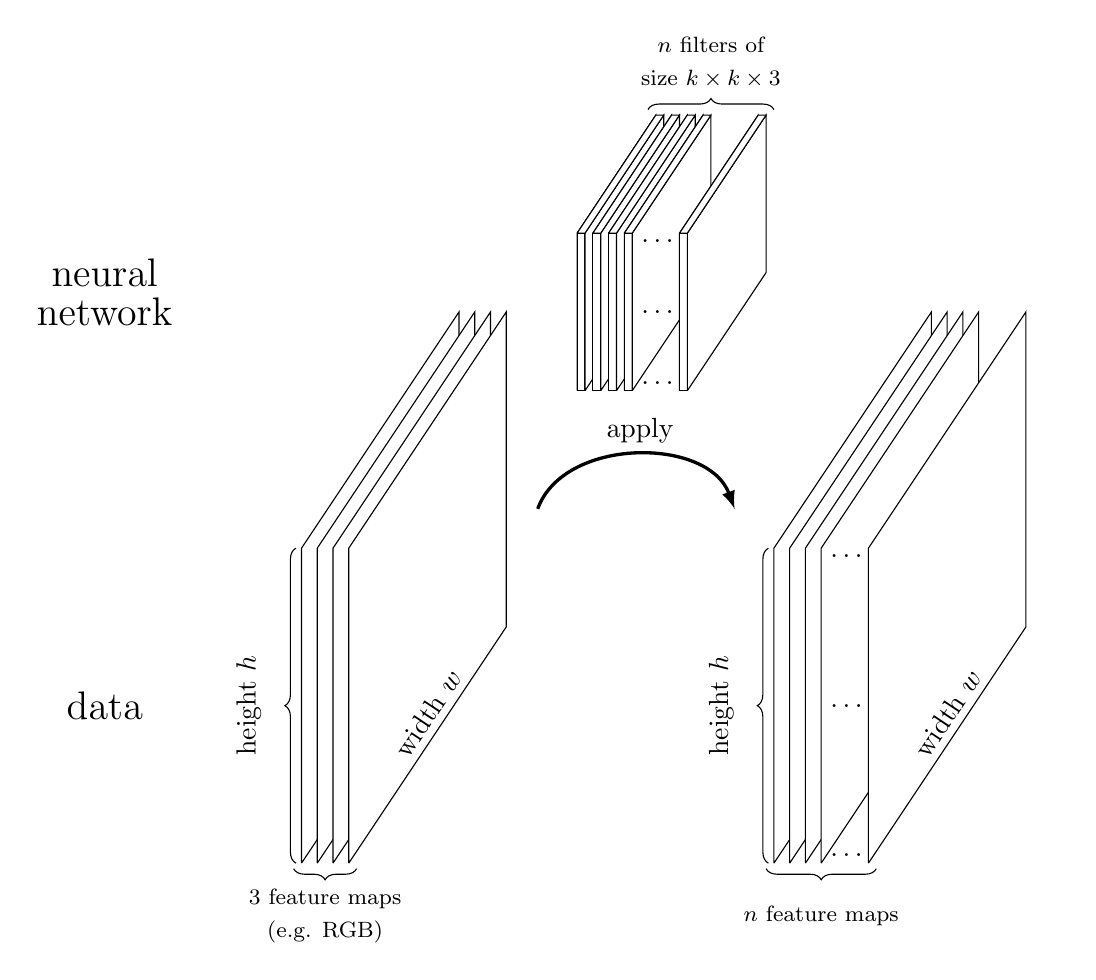
\begin{tikzpicture}
    % Print input feature maps
    \foreach \i in {0, 0.2, ..., 0.6} {
        \draw[fill=white] (0+\i, 0) -- (2+\i, 3) -- (2+\i, 7) -- (\i, 4) -- (\i, 0);
    }

    % Print filters
    \foreach \i in {0, 0.2, ..., 0.6, 1.3} {
        \draw[fill=white] (\xup+\i, \yup) -- (\xup+\upsizex+\i, \yup+\upshift) -- (\xup+\upsizex+\i, \yup+\upsizey+\upshift) -- (\xup+\i, \yup+\upsizey) -- (\xup+\i, \yup);
        \draw[fill=white] (\xup+\i, \yup) -- (\xup+\i+0.1, \yup) -- (\xup+\i+0.1, \yup+\upsizey) -- (\xup+\i, \yup+\upsizey) -- (\xup+\i, \yup);
        \draw[fill=white] (\xup+\i+0.1, \yup) -- (\xup+\upsizex+\i+0.1, \yup+\upshift) -- (\xup+\upsizex+\i+0.1, \yup+\upsizey+\upshift) -- (\xup+\i+0.1, \yup+\upsizey) -- (\xup+\i+0.1, \yup);
        \draw[fill=white] (\xup+\i, \yup+\upsizey) -- (\xup+\i+0.1, \yup+\upsizey) -- (\xup+\upsizex+\i+0.1, \yup+\upsizey+\upshift) -- (\xup+\upsizex+\i, \yup+\upsizey+\upshift) -- (\xup+\i, \yup+\upsizey);
    }

    \foreach \i in {0, 0.2, ..., 0.6, 1.2} {
        \draw[fill=white] (\distance+\i, 0) -- (\distance+2+\i, 3) -- (\distance+2+\i, 7) -- (\distance+\i, 4) -- (\distance+\i, 0);
    }

    \draw [decorate,decoration={brace,amplitude=+4pt,mirror},xshift=0pt,yshift=-2pt]
(-0.1,0) -- (0.7,0) node [black,midway,yshift=-0.6cm, align=center] {\footnotesize$3$ feature maps\\\footnotesize(e.g. RGB)};
    \draw [decorate,decoration={brace,amplitude=+4pt,mirror},xshift=0pt,yshift=-2pt]
(\distance-0.1,0) -- (\distance+1.3,0) node [black,midway,yshift=-0.6cm, align=center] {\footnotesize$n$ feature maps};
    \draw [decorate,decoration={brace,amplitude=+4pt},xshift=0pt,yshift=+2pt]
(\xup-0.1+\upsizex,\yup+\upsizey+\upshift) -- (\xup+1.5+\upsizex,\yup+\upsizey+\upshift) node [black,midway,yshift=+0.6cm, align=center] {\footnotesize $n$ filters of\\\footnotesize size $k \times k \times 3$};
    \draw[very thick, ->,>=latex] (3, 4.5) [out=70, in=110] to  (\distance-0.5, 4.5);
    \draw [color=white,decorate,decoration={brace,amplitude=+4pt, mirror},xshift=0pt,yshift=+2pt]
(1.1, 0) -- (3.1, 3) node [sloped,black,midway,yshift=+0.6cm, align=center] {width $w$};
    \draw [color=white,decorate,decoration={brace,amplitude=+4pt, mirror},xshift=0pt,yshift=+2pt]
(\distance+1.7, 0) -- (\distance+3.7, 3) node [sloped,black,midway,yshift=+0.6cm, align=center] {width $w$};
    \draw [decorate,decoration={brace,amplitude=+4pt},xshift=-2pt,yshift=0pt]
(0, 0) -- (0, 4) node [sloped,black,midway,yshift=+0.6cm, align=center] {height $h$};
    \draw [decorate,decoration={brace,amplitude=+4pt},xshift=-2pt,yshift=0pt]
(\distance, 0) -- (\distance, 4) node [sloped,black,midway,yshift=+0.6cm, align=center] {height $h$};
    \node at (-2.5,7.5) {\Large neural};
    \node at (-2.5,7) {\Large network};
    \node at (-2.5,2) {\Large data};

    \node at (+4.3,5.5) {apply};
    \node at (\distance+0.95,3.9) {\dots};
    \node at (\distance+0.95,2) {\dots};
    \node at (\distance+0.95,0.1) {\dots};

    \node at (\xup+1.05,\yup+1.9) {\dots};
    \node at (\xup+1.05,\yup+1.0) {\dots};
    \node at (\xup+1.05,\yup+0.1) {\dots};
\end{tikzpicture}
